\section{Theoretischer Hintergrund des Versuches}
\label{sec:Theorie}
\subsection{Eigenschaften des Myons}
\label{subsec:Eigenschaften}
Myonen sind Leptonen aus der zweiten der drei Leptonenfamilien. Sie haben
eine Ruhemasse von $\SI{105.66}{\mega\electronvolt}$ sowie eine Lebensdauer
von $\SI{2.197}{\micro\second}$. Das Myon $\mu^{-}$ ist einfach negativ geladen,
das Antimyon $\mu^{+}$ daher einfach positiv.\cite{PDG}
Myonen unterliegen wie alle Fermionen der schwachen und der elektromagnetischen
Wechselwirkung.
\subsection{Enstehung von kosmischer Strahlung}
\label{subsec:kosmischeStrahlung}
Als primäre kosmische Strahlung werden hochenergetische Teilchen bezeichnet, welche
in der Sonne und anderen Sternen entstanden sind. Sie besteht hauptsächlich aus Protonen.
Diese wechselwirken mit Teilchen in der Atmosphäre, was elektromagnetische
Schauer erzeugt. In diesen Schauern entstehen Sekundärteilchen. Bei diesen
Sekundärteilchen handelt es sich hauptsächlich um Pionen und Kaonen.
\begin{figure}
  \centering
  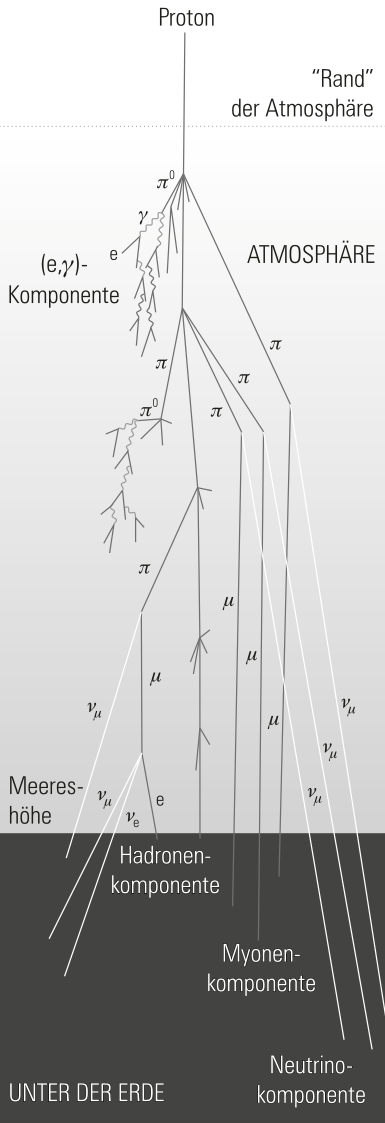
\includegraphics[width=0.2\textwidth]{pictures/Schauer.png}
  \caption{Schematische Darstellung eines EM-Schauers kosmischer Strahlung. \cite{Q1}}
  \label{fig:schauer}
\end{figure}
\noindent
Die so enstandenen Pionen zerfallen aufgrund der Helizitätsunterdrückung
des Zerfalls
\begin{align*}
  \pi^{-} & \rightarrow e^{-} + \bar{\nu}_{e} \\
  \pi^{+} & \rightarrow e^{+} + \nu_{e}
\end{align*}
\noindent
hauptsächlich über die Zerfallskanäle
\begin{align*}
\pi^{-} & \rightarrow \mu^{-} + \bar{\nu}_{\mu} \\
\pi^{+} & \rightarrow \mu^{+} + \nu_{\mu}.
\end{align*}
\noindent
Der Zerfall der Kaonen verhält sich analog. Die aus kosmischer Strahlung entstandenen
Myonen werden kosmische Myonen genannt.
Sie zerfallen, wie in Abbildung \ref{zerfall} dargestellt, über die schwache Wechselwirkung.
\begin{figure}[H]
  \centering
  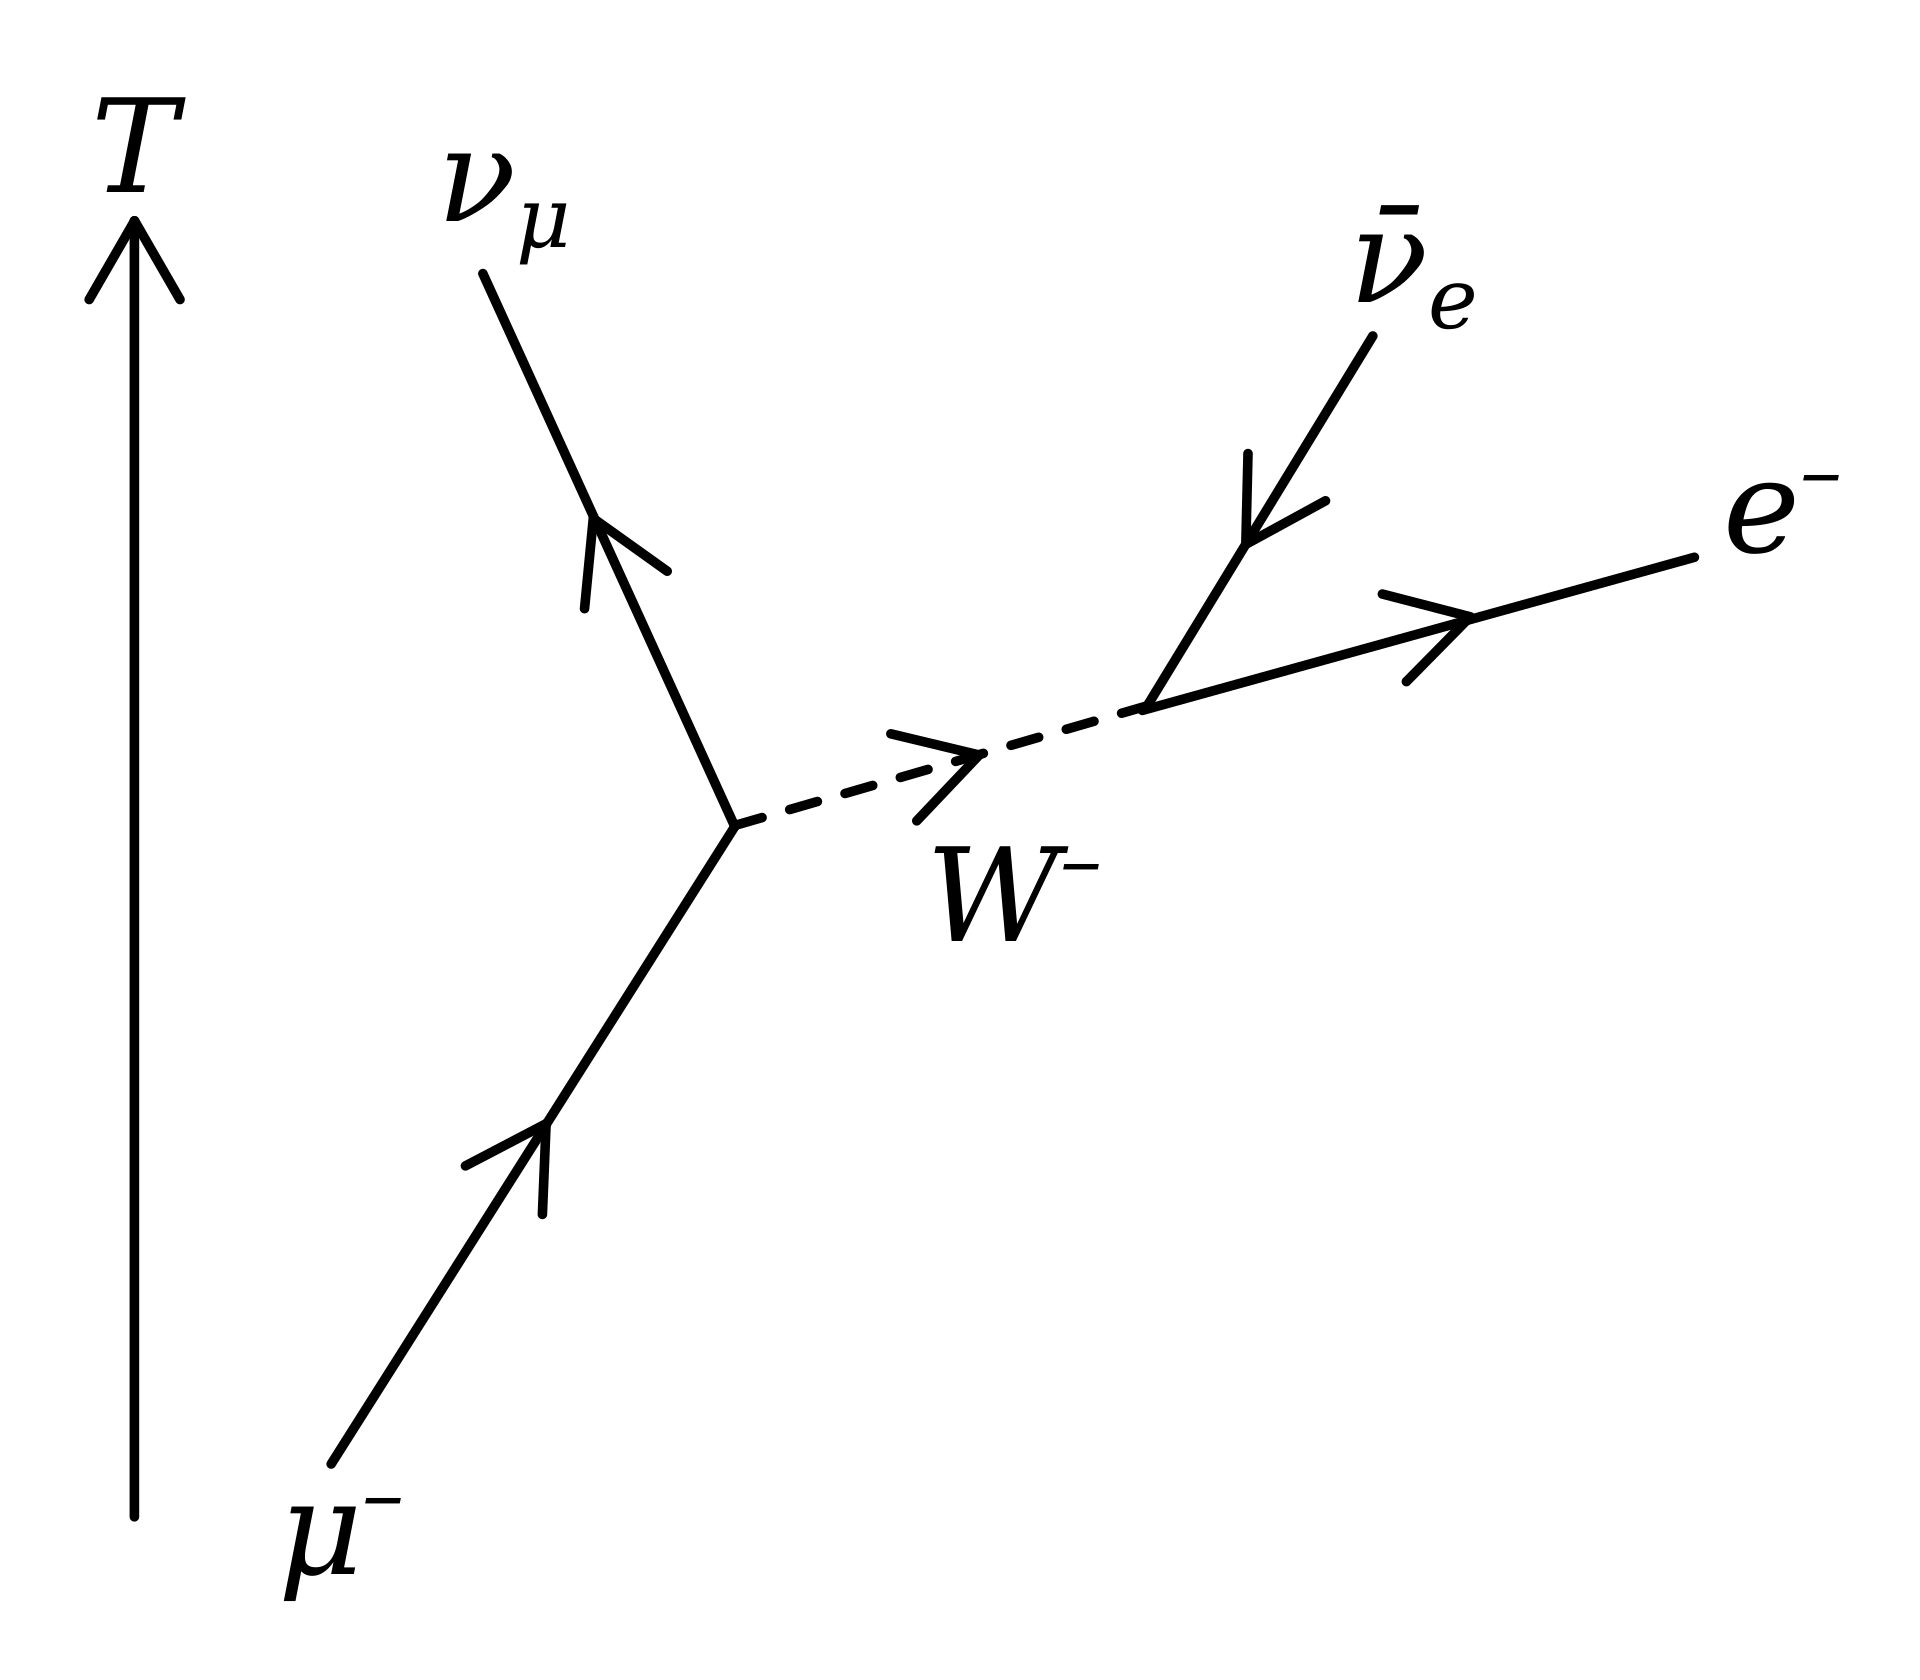
\includegraphics[width=0.5\textwidth]{pictures/Muon_Decay.png}
  \caption{Feynman-Graph des Myonenzerfalls.\cite{Myon-Wikipedia}}
  \label{zerfall}
\end{figure}
\noindent
Teilchenzerfälle sind statistische Prozesse. Daher wird dem Zerfall des Myons
eine Wahrscheinlichkeit $\text{d}W$  zugeordnet, mit der dieser in einer bestimmten Zeit $\text{d}t$
stattfindet:
\begin{equation*}
  \text{d}W = \lambda \text{d}t.
\end{equation*}
\noindent
Hierbei ist der Proportionalitätsfaktor $\lambda$ die Zerfallskonstante.
Die Zerfallskonstante und die mittlere Lebensdauer eines Teilchens haben den folgenden
Zusammenhang:
\begin{equation*}
  \lambda = \frac{1}{\tau}.
\end{equation*}
\noindent
Die mittlere Lebensdauer beschreibt die Zeit, nach der sich die Anzahl der Teilchen um
den Faktor $e \approx 2.7$ verringert hat.
Für die Änderung der Teilchenzahl $N$ in einem Zeitraum $\text{d}t$ gilt
\begin{equation}
  \text{d}N = - N \cdot \text{d}W = - N \cdot \lambda \text{d}t.
  \label{eqn:zerfall1}
\end{equation}
\noindent
Durch Integration der Gleichung \ref{eqn:zerfall1} kann das Zerfallsgesetz hergeleitet werden:
\begin{equation}
  N(t) = N_{0} \cdot \exp{(-\lambda t)}.
  \label{eqn:zerfallsgesetz}
\end{equation}
\noindent
\subsection{Bestimmung der mittleren Lebensdauer der Myonen}
\label{subsec:BestimmungLebensdauer}
Um die kosmischen Myonen zu detektieren, wird ein organischer Szintillator verwendet.
Szintillatoren erzeugen bei Eintritt eines geladenen Teilchens einen Lichtpuls.
Dieser entsteht, da durch Eintritt eines geladenen Teilchens Moleküle des Szintillators
angeregt werden, welche dann unter Abgabe von Photonen wieder in ihre Grundzustände zurückfallen.
Diese Lichtpulse können in elektrische Signale umgewandelt und weiterverarbeitet werden.
Bei Eintritt eines Myons in den Szintillator wird ein Signal gemessen. Wenn das Myon innerhalb
des Szintillators, wie in der Abbildung \ref{zerfall} dargestellt, zerfällt, kann auch von den Zerfallsprodukten
ein Signal detektiert werden. Dies ist der Fall, wenn das Myon seine gesamte kinetische Energie
an das Szintillatormaterial abgibt.
Durch Messung der Zeit zwischen dem Eintritt des Myons und des
Zerfalls ist eine Bestimmung der mittleren Lebensdauer des Myons möglich. Es wird also
innerhalb eines bestimmten Zeitrahmens nach Eintritt eines Myons auf ein weiteres Signal
gewartet. Wenn innerhalb dieses Zeitrahmens ein weiteres Myon den Detektor erreicht oder wenn
ein Myon nicht innerhalb des Detektors zerfällt, kann die Messung verfälscht werden, da
Zerfälle, welche außerhalb des Messzeitrahmens stattfinden, nicht gemessen werden.
Diese Verfälschungen der Messung erzeugen einen Untergrund. Dieser lässt sich mithilfe
einer Poissonverteilung abschätzen. Dies ist in folgender Gleichung angegeben:
\begin{equation}
  U = P_{\lambda} (k) = \frac{\lambda^{k}}{k!} \exp{(-\lambda)},
  \label{eqn:Untergrundrate}
\end{equation}
\noindent
mit dem Erwartungswert der Poissonverteilung $\lambda$ und der Ereignisanzahl $k$.
